\chapter{Attention That Pervades Life}

This chapter follows J. Krishnamurti's San Diego dialogue with Dr. Alan W. Anderson on meditation as a quality of attention that is not separate from life. The source material is credited to J. Krishnamurti and the Krishnamurti Foundation Trust; this course-book curation is by LazyingArt LLC. There are no validated blackboard frames for this lecture, so the equations and diagrams below are not board transcriptions. They are compact reconstructions of the dialogue's logical movement: arrows mark sequence, implications mark conceptual pressure, and the prose remains the primary source of meaning.

\section{Beginning Without A Method}

Anderson begins where the previous conversation had left off: the dialogue is ready to take up meditation. The expected opening would be a practical one: Which meditation is right? Which school, which discipline, which form of prayer, which method? Krishnamurti refuses that opening. Before there can be a method, there must be a question. What is meditation?

He names the inherited field first. There are Hindu, Buddhist, Christian, Sufi, Zen, and imported guru traditions. There are prayers repeated endlessly, mantras whispered or sounded inwardly, breathing systems, vows, disciplines, and routines. Krishnamurti is not pretending that these do not exist. He is asking whether beginning from any of them already places the mind inside tradition.

The first real step is therefore not an answer but a clearing:

\begin{definition}[Starting from not-knowing]
In this dialogue, not-knowing is not confusion. It is freedom from borrowed conclusions, inherited practices, spiritual authority, and another person's experience of illumination.
\end{definition}

The structure is simple enough to write as a schematic equation:

\begin{equation}
\text{not-knowing}
\longrightarrow
\text{freedom from the established known}
\longrightarrow
\text{inquiry}.
\end{equation}

This is the first point to preserve. Meditation is not introduced as a technique. It begins when the mind is free enough to ask without already leaning on a conclusion.

\section{Tradition, Practice, And The Static Goal}

Krishnamurti next examines what is hidden inside practice. Suppose there is a mantra, a prayer, a breathing discipline, a repeated posture, or a system passed down by a teacher. The practice may appear humble, patient, and serious. Yet if it is undertaken in order to arrive at truth, God, enlightenment, or some ultimate state, then the destination has already been projected.

The usual structure is

\begin{equation}
\text{practice}
\longrightarrow
\text{imagined goal}.
\end{equation}

Anderson sharpens this by distinguishing two kinds of activity: one whose end lies outside the activity, and one whose end is intrinsic to the act itself. Krishnamurti accepts the distinction. A path toward a goal treats the goal as already known enough to be reached. It turns the living into something fixed.

\begin{equation}
\text{practice toward truth}
\Rightarrow
\text{truth treated as fixed, static, and already pictured}.
\end{equation}

That is the hidden contradiction. If truth is living, then it cannot be approached as a dead point at the end of a road. The mind may become quiet through repetition, but a quietness produced by routine may also be mechanical. Krishnamurti's word for this danger is dullness: practice, practice, practice, and the mind becomes conditioned by its own repetition.

\subsection{Question \& Answer}

\paragraph{Question.}
If practice aims at truth, must truth be treated as fixed?

\paragraph{Answer.}
In the logic of the dialogue, yes. A practice organized as a route to a promised destination has already imagined the destination. It may call the destination truth, God, enlightenment, or grace, but the structure is the same. The mind is moving toward an image. Krishnamurti therefore shifts the inquiry from ``How shall we meditate?'' to ``What is meditation?''

\begin{figure}
\centering
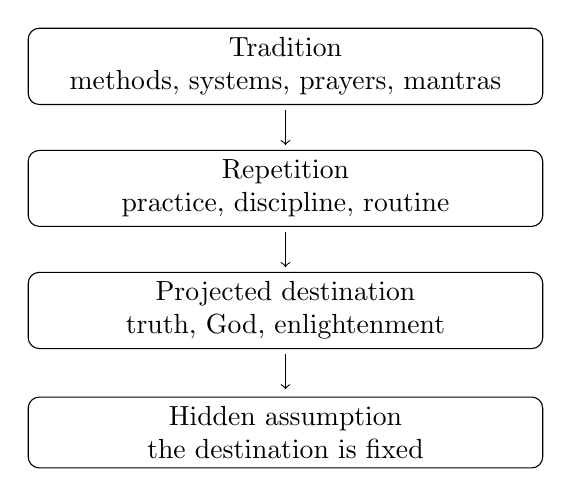
\begin{tikzpicture}[x=1cm,y=1cm]
\node[draw, rounded corners, align=center, text width=6.3cm] at (0,0)
{Tradition\\methods, systems, prayers, mantras};
\node[draw, rounded corners, align=center, text width=6.3cm] at (0,-1.55)
{Repetition\\practice, discipline, routine};
\node[draw, rounded corners, align=center, text width=6.3cm] at (0,-3.10)
{Projected destination\\truth, God, enlightenment};
\node[draw, rounded corners, align=center, text width=6.3cm] at (0,-4.65)
{Hidden assumption\\the destination is fixed};
\draw[->] (0,-0.55) -- (0,-1.00);
\draw[->] (0,-2.10) -- (0,-2.55);
\draw[->] (0,-3.65) -- (0,-4.10);
\end{tikzpicture}
\end{figure}

The figure is a reader's diagram, not a board reconstruction. Its purpose is to keep the inference visible: method implies goal; goal implies projection; projection makes the living thing static.

\section{Meditation And The Whole Field Of Life}

After the inherited paths have been put aside, Krishnamurti asks the first positive test. Is meditation divorced from daily living? The rhythm of the dialogue matters here. He does not define meditation abstractly and then apply it to life. He turns immediately to conduct, desire, ambition, greed, envy, competition, imitation, conformity, pleasure, sex, anxiety, fear, death, and relationship. If meditation does not include these, it is an escape from the field in which human beings actually live.

The contrast can be written compactly:

\begin{align}
\text{meditation} &\neq \text{escape from daily living},\\
\text{meditation} &\supset
\{\text{conduct}, \text{desire}, \text{pleasure}, \text{fear},
\text{death}, \text{relationship}, \text{work}\}.
\end{align}

Here \(\supset\) is only a schematic sign. It means that meditation, if the word is to have weight, must include the field of life rather than float above it. A private inward state, a protected hour, or a sacred technique that leaves conduct unchanged is still a division.

Anderson's theological reflections enter at this point as a genuine part of the dialogue. He brings in the Jesus Prayer, the finite character of repeated words, and the question of whether religious language can be understood as living action rather than doctrine. Krishnamurti does not turn the conversation into comparative religion. He keeps pressing the structure: repetition conditions, belief carries tradition, a path assumes a fixed end, and meditation cannot be separate from living.

\begin{table}
\centering
\begin{tabular}{p{0.42\linewidth}p{0.42\linewidth}}
\hline
Path or method & Inquiry beginning in freedom \\
\hline
Starts from inherited authority & Starts from ``I do not know'' \\
Repeats a word, prayer, or system & Looks directly at life as it is \\
Moves toward an imagined end & Lets the question unfold in the act \\
Risks mechanical dullness & Requires sensitive attention \\
\hline
\end{tabular}
\end{table}

This table is deliberately plain. Its function is not to classify traditions, but to show the hinge of the lecture: meditation is either added to life as a practice, or it is inseparable from the whole movement of life.

\section{Seeing The False And The Fragmented}

The next movement is from method to perception. Krishnamurti does not ask us to condemn a practice because he condemns it. He says the false must be seen. The eyes must look without prejudice and without reaction. Then the falseness or truth of a thing is revealed in the perception itself.

\begin{equation}
\text{looking without prejudice or reaction}
\longrightarrow
\text{the false seen as false}.
\end{equation}

The test remains concrete. A person may claim to be full of love, truth, knowledge, or wisdom. Krishnamurti asks a simpler question: how does that person live? Is there freedom from fear, ambition, greed, envy, and the desire to succeed in every field? If not, the claim is only a performance.

This is why the dialogue moves naturally into fragmentation. Meditation includes the whole field of existence; therefore it includes the social and professional divisions by which human beings define themselves. Artist, businessperson, politician, priest, scholar, scientist: these are not treated here as neutral job titles. They are signs of a consciousness that has divided itself and then expressed its division outwardly.

\begin{equation}
\text{fragmented human being}
\longrightarrow
\{\text{artist}, \text{businessperson}, \text{politician},
\text{priest}, \text{scholar}, \text{scientist}\}.
\end{equation}

\subsection{Question \& Answer}

\paragraph{Question.}
Can art, scholarship, or science be whole if the human being is fragmented?

\paragraph{Answer.}
Not in this inquiry. The artist may be sensitive to beauty and nature; the scholar may be disciplined; the scientist may be exact. But if the human being is inwardly divided, the special role does not heal the division. Krishnamurti's order is exact: first there must be a total human being; then what is created or done may have beauty.

\begin{figure}
\centering
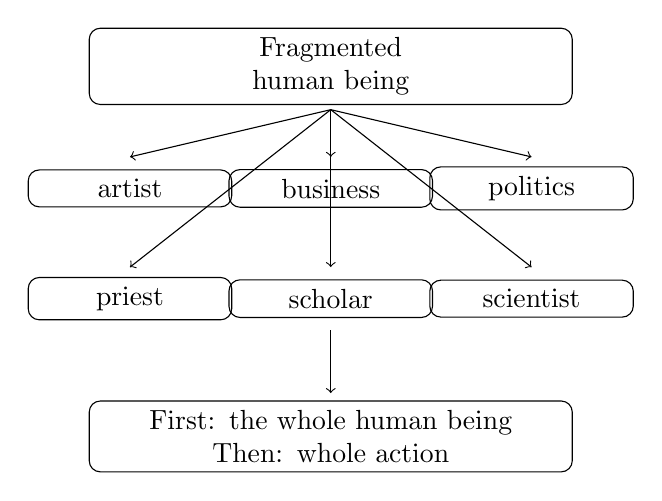
\begin{tikzpicture}[x=1cm,y=1cm]
\node[draw, rounded corners, align=center, text width=5.9cm] at (0,0)
{Fragmented\\human being};
\node[draw, rounded corners, align=center, text width=2.35cm] at (-2.55,-1.55) {artist};
\node[draw, rounded corners, align=center, text width=2.35cm] at (0,-1.55) {business};
\node[draw, rounded corners, align=center, text width=2.35cm] at (2.55,-1.55) {politics};
\node[draw, rounded corners, align=center, text width=2.35cm] at (-2.55,-2.95) {priest};
\node[draw, rounded corners, align=center, text width=2.35cm] at (0,-2.95) {scholar};
\node[draw, rounded corners, align=center, text width=2.35cm] at (2.55,-2.95) {scientist};
\node[draw, rounded corners, align=center, text width=5.9cm] at (0,-4.70)
{First: the whole human being\\Then: whole action};
\draw[->] (0,-0.55) -- (-2.55,-1.15);
\draw[->] (0,-0.55) -- (0,-1.15);
\draw[->] (0,-0.55) -- (2.55,-1.15);
\draw[->] (0,-0.55) -- (-2.55,-2.55);
\draw[->] (0,-0.55) -- (0,-2.55);
\draw[->] (0,-0.55) -- (2.55,-2.55);
\draw[->] (0,-3.35) -- (0,-4.15);
\end{tikzpicture}
\end{figure}

This is not a moral ranking of professions. It is a map of the argument. A divided mind can turn even beauty, learning, or religion into another fragment.

\section{Freedom As The Energy Of Inquiry}

At this point the lecture recaps itself. Systems, methods, gurus, authorities, beliefs, and hopes have been seen as burdens. To discard them is not merely to negate. It releases the energy to inquire.

\begin{equation}
\text{discarded burden}
\longrightarrow
\text{freedom}
\longrightarrow
\text{energy for inquiry}.
\end{equation}

This is where the earlier ``I do not know'' returns with greater force. It is not a slogan. It is the condition in which the mind is not asking another person, another book, another professor, another psychologist, another tradition, to supply the answer. Krishnamurti insists that the mind capable of real inquiry begins with humility, not with accumulated authority.

We can collect the argument so far as a worked derivation.

\begin{proposition}[The burden of method]
If meditation is approached as a method leading to a projected end, then the inquiry is already burdened by an image of that end.
\end{proposition}

\begin{proof}
A method is practiced in order to arrive somewhere. If the destination is to be reached by practice, the destination must already be pictured or promised. A pictured destination is no longer an unknown living truth, but a fixed object of pursuit. Therefore the mind following method is also carrying the authority, hope, and belief attached to that method. To inquire freely, the mind must see and put aside that burden. It then begins again from not-knowing.
\end{proof}

The proof is not offered as formal philosophy. It is a clean reconstruction of the lecture's sequence. It also prepares the next question. If meditation includes the whole field of life, it must include sleep, waking, knowledge, and the past.

\section{Awake, Asleep, And The Past}

Krishnamurti now turns to sleep, but he does not begin with dreams. He begins with waking. What does it mean to be awake? Not merely awake to public events, politics, economics, or social disturbances. Awake means sensitive to what is happening inwardly and outwardly. It cannot be episodic. It cannot depend on crisis, shock, challenge, or stimulation.

The negative structure is useful:

\begin{align}
\text{stimulation} &\neq \text{wakefulness},\\
\text{fear, illusion, or burden} &\Rightarrow \text{not awake}.
\end{align}

Anderson's example of an animal completely looking and completely sleeping serves as a conversational bridge. Krishnamurti accepts the point, but he brings the inquiry back to the human problem: is the past so alive that it dictates life in the present?

Here the distinction must be kept sharp. The past is necessary as knowledge. We need knowledge for language, skill, work, direction, and practical functioning. But when the past covers the present, when old hurt, failure, depression, conclusion, and experience speak in place of direct perception, then one is asleep now.

\begin{align}
\text{past as knowledge} &= \text{necessary},\\
\text{past covering the present} &\Rightarrow \text{not awake}.
\end{align}

\subsection{Question \& Answer}

\paragraph{Question.}
Can the past function as knowledge without dominating the present?

\paragraph{Answer.}
That is the subtle balance Krishnamurti is asking us to see. Knowledge must function where knowledge is required. But if the past overflows into the present and interprets everything before it is seen, the mind is no longer awake. Awareness and knowledge must move without contradiction: knowledge operating in its proper field, attention awake to what is actually taking place.

\begin{equation}
\text{awareness} + \text{knowledge in its proper field}
\longrightarrow
\text{balance without contradiction}.
\end{equation}

Anderson names this as a relation between knowing and understanding. Krishnamurti accepts it as part of meditation and immediately presses onward. If this is what it means to be awake, then what is sleep?

\section{Dreams, Order, And The Rested Brain}

The question of sleep is approached in the same way as meditation itself: not from authorities, but from direct inquiry. What are dreams? Why should the mind dream? Krishnamurti's answer is not a theory of dream symbolism. It is a continuation of the question of disorder.

If daily life is unwatched, if its disorder is not understood, that disorder continues into sleep. The brain requires order in order to function. If order has not been found during the day, the brain tries to bring order during the night, through dreams or intimations.

\begin{align}
\text{daily disorder unwatched}
&\longrightarrow
\text{disorder continues in sleep}
\longrightarrow
\text{dreams},\\
\text{daily disorder understood}
&\longrightarrow
\text{order during waking}
\longrightarrow
\text{quiet sleep}
\longrightarrow
\text{rest}.
\end{align}

This should not be expanded into neuroscience. The terms are Krishnamurti's terms: order, disorder, quietness, conflict, rest, regeneration. The claim is that order during waking changes the quality of sleep. If the mind has watched disorder during the day and understood it, the brain need not labor at night to establish security through dreams.

\subsection{Question \& Answer}

\paragraph{Question.}
Are all dreams merely unfinished disorder?

\paragraph{Answer.}
Anderson asks about dreams that seem to point to a future event. Krishnamurti answers with an image: from high in the hills, one can see two boats moving on a river and know where they will meet. That is not prediction by fantasy; it is seeing from a wider vantage. Anderson distinguishes this from subjective unfinished business. The main line remains: the dreams under discussion are the continuation of daily disorder that has not been understood.

\begin{figure}
\centering
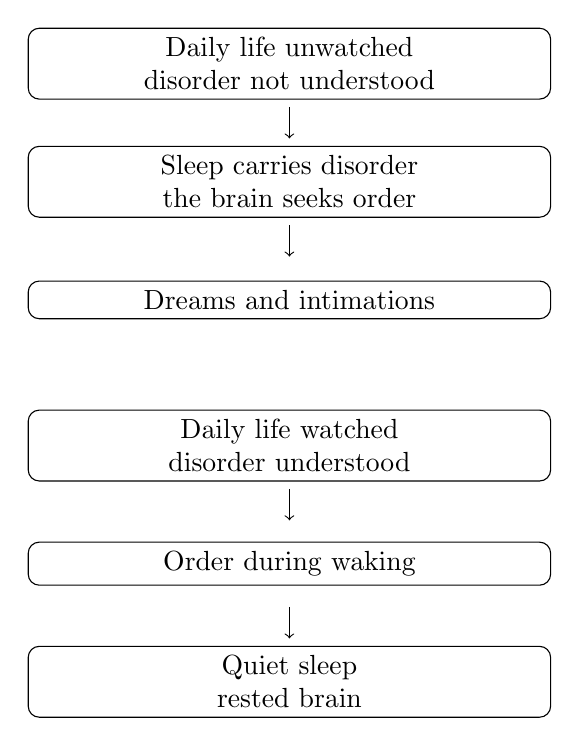
\begin{tikzpicture}[x=1cm,y=1cm]
\node[draw, rounded corners, align=center, text width=6.4cm] at (0,0)
{Daily life unwatched\\disorder not understood};
\node[draw, rounded corners, align=center, text width=6.4cm] at (0,-1.50)
{Sleep carries disorder\\the brain seeks order};
\node[draw, rounded corners, align=center, text width=6.4cm] at (0,-3.00)
{Dreams and intimations};
\node[draw, rounded corners, align=center, text width=6.4cm] at (0,-4.85)
{Daily life watched\\disorder understood};
\node[draw, rounded corners, align=center, text width=6.4cm] at (0,-6.35)
{Order during waking};
\node[draw, rounded corners, align=center, text width=6.4cm] at (0,-7.85)
{Quiet sleep\\rested brain};
\draw[->] (0,-0.55) -- (0,-0.95);
\draw[->] (0,-2.05) -- (0,-2.45);
\draw[->] (0,-5.40) -- (0,-5.80);
\draw[->] (0,-6.90) -- (0,-7.30);
\end{tikzpicture}
\end{figure}

After this, Krishnamurti asks whether the mind lives in that quality during the day. If not, it is not meditation. The inquiry into sleep returns us to waking life.

\section{Control, Desire, And Flowering}

The final movement begins with another inherited command: control. Religions have said to control desire, thought, impulse, and the self. Krishnamurti does not simply reject discipline in favor of disorder. He asks what control is and who the controller is.

The central identity is stated with unusual force:

\begin{equation}
\text{controller} = \text{controlled}.
\end{equation}

When one says, ``I must control my thought,'' the controller is itself a movement of thought. Thought then controls thought; one fragment controls another fragment; fragmentation remains.

\begin{equation}
\text{thought controls thought}
\Rightarrow
\text{one fragment controls another}
\Rightarrow
\text{fragmentation remains}.
\end{equation}

\subsection{Question \& Answer}

\paragraph{Question.}
Can there be a life of meditation without control?

\paragraph{Answer.}
Krishnamurti's answer is not indulgence. The question is whether there is order without suppression. Anderson names the point: when intelligence breaks out, order comes with it. Krishnamurti goes further: intelligence is order; the seeing is the doing. Control belongs to division. The inquiry therefore has to be tested in the concrete movement of desire.

Desire arises in sequence:

\begin{equation}
\text{seeing}
\longrightarrow
\text{contact}
\longrightarrow
\text{sensation}
\longrightarrow
\text{desire}.
\end{equation}

Once desire has arisen, there are three visible movements:

\begin{equation}
\text{desire}
\longrightarrow
\{\text{suppression},\ \text{yielding},\ \text{flowering under watchfulness}\}.
\end{equation}

Suppression is control; yielding fragments life into getting and losing. The third movement is the difficult one: desire is allowed to flower while it is watched, neither resisted nor obeyed. Krishnamurti's claim is that in this complete watchfulness the flowering itself is the ending of that desire.

\begin{equation}
\text{desire observed without control}
\longrightarrow
\text{flowering}
\longrightarrow
\text{ending}.
\end{equation}

\begin{figure}
\centering
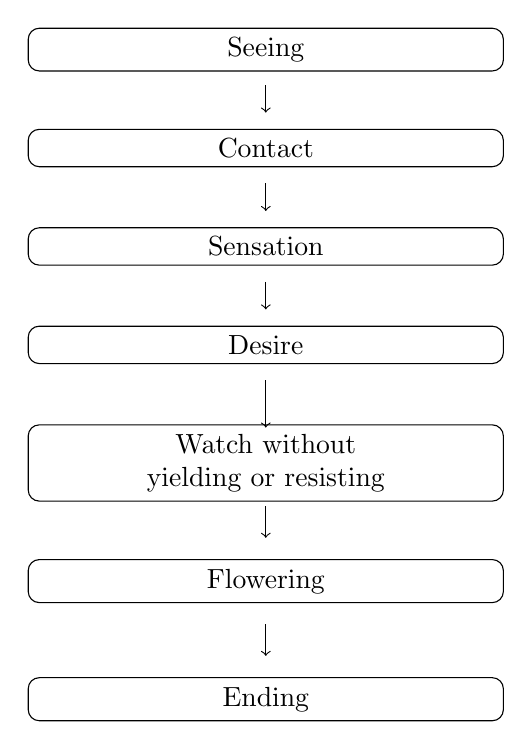
\begin{tikzpicture}[x=1cm,y=1cm]
\node[draw, rounded corners, align=center, text width=5.8cm] at (0,0)
{Seeing};
\node[draw, rounded corners, align=center, text width=5.8cm] at (0,-1.25)
{Contact};
\node[draw, rounded corners, align=center, text width=5.8cm] at (0,-2.50)
{Sensation};
\node[draw, rounded corners, align=center, text width=5.8cm] at (0,-3.75)
{Desire};
\node[draw, rounded corners, align=center, text width=5.8cm] at (0,-5.25)
{Watch without\\yielding or resisting};
\node[draw, rounded corners, align=center, text width=5.8cm] at (0,-6.75)
{Flowering};
\node[draw, rounded corners, align=center, text width=5.8cm] at (0,-8.25)
{Ending};
\draw[->] (0,-0.45) -- (0,-0.80);
\draw[->] (0,-1.70) -- (0,-2.05);
\draw[->] (0,-2.95) -- (0,-3.30);
\draw[->] (0,-4.20) -- (0,-4.80);
\draw[->] (0,-5.80) -- (0,-6.20);
\draw[->] (0,-7.30) -- (0,-7.70);
\end{tikzpicture}
\end{figure}

This is where the lecture deliberately stops. Anderson notices the plant image and asks to continue with it in the next conversation. Krishnamurti agrees. Meditation has not been completed as a topic; attention has only been opened into the next question.

\section{Summary}

The movement of the chapter is a clearing and then a widening. Meditation is not first a method, a prayer, a mantra, a system, or a route toward a projected goal. Such a route already imagines the destination and so makes truth static. Krishnamurti begins instead with not-knowing: a freedom from the burden of inherited answers.

From there the inquiry widens into the whole field of living. Meditation must include conduct, desire, pleasure, fear, death, relationship, work, art, and the fragmented roles through which human beings divide themselves. It must include waking and sleep. Knowledge is necessary, but when the past covers the present, the mind is asleep. Dreams continue disorder when daily disorder has not been understood; order during waking permits quiet sleep and rest.

The final question is control. If the controller is the controlled, control is one fragment acting on another. Desire then becomes the concrete test: seeing, contact, sensation, desire, and then not suppression, not yielding, but watchfulness in which desire flowers and ends. The dialogue closes without finality, which is fitting. Meditation, in this conversation, is not a conclusion but attention that must pervade life.